\documentclass[letterpaper,12pt]{article}
\usepackage[margin=.65in,top=.72in,bottom=.62in,headheight=16pt,headsep=15pt,footskip=19pt]{geometry}
\usepackage[T1]{fontenc}
\usepackage{lmodern,tikz,fancyhdr}\pdfmapfile{+lm.map}
\usetikzlibrary{arrows.meta,shapes.geometric}
\pagestyle{fancy}\fancyhf{}\renewcommand{\headrulewidth}{0pt}\renewcommand{\footrulewidth}{0pt}
\setlength{\parindent}{0pt}\setlength{\parskip}{0pt}
\fancyhead[L]{\small Week 44 / The bag that copies / Grades 2--3}
\fancyfoot[L]{\footnotesize Bellingham Math Circle / Week 44 / W44-grades-2-3-v2}\fancyfoot[R]{\footnotesize\thepage}
\begin{document}
\noindent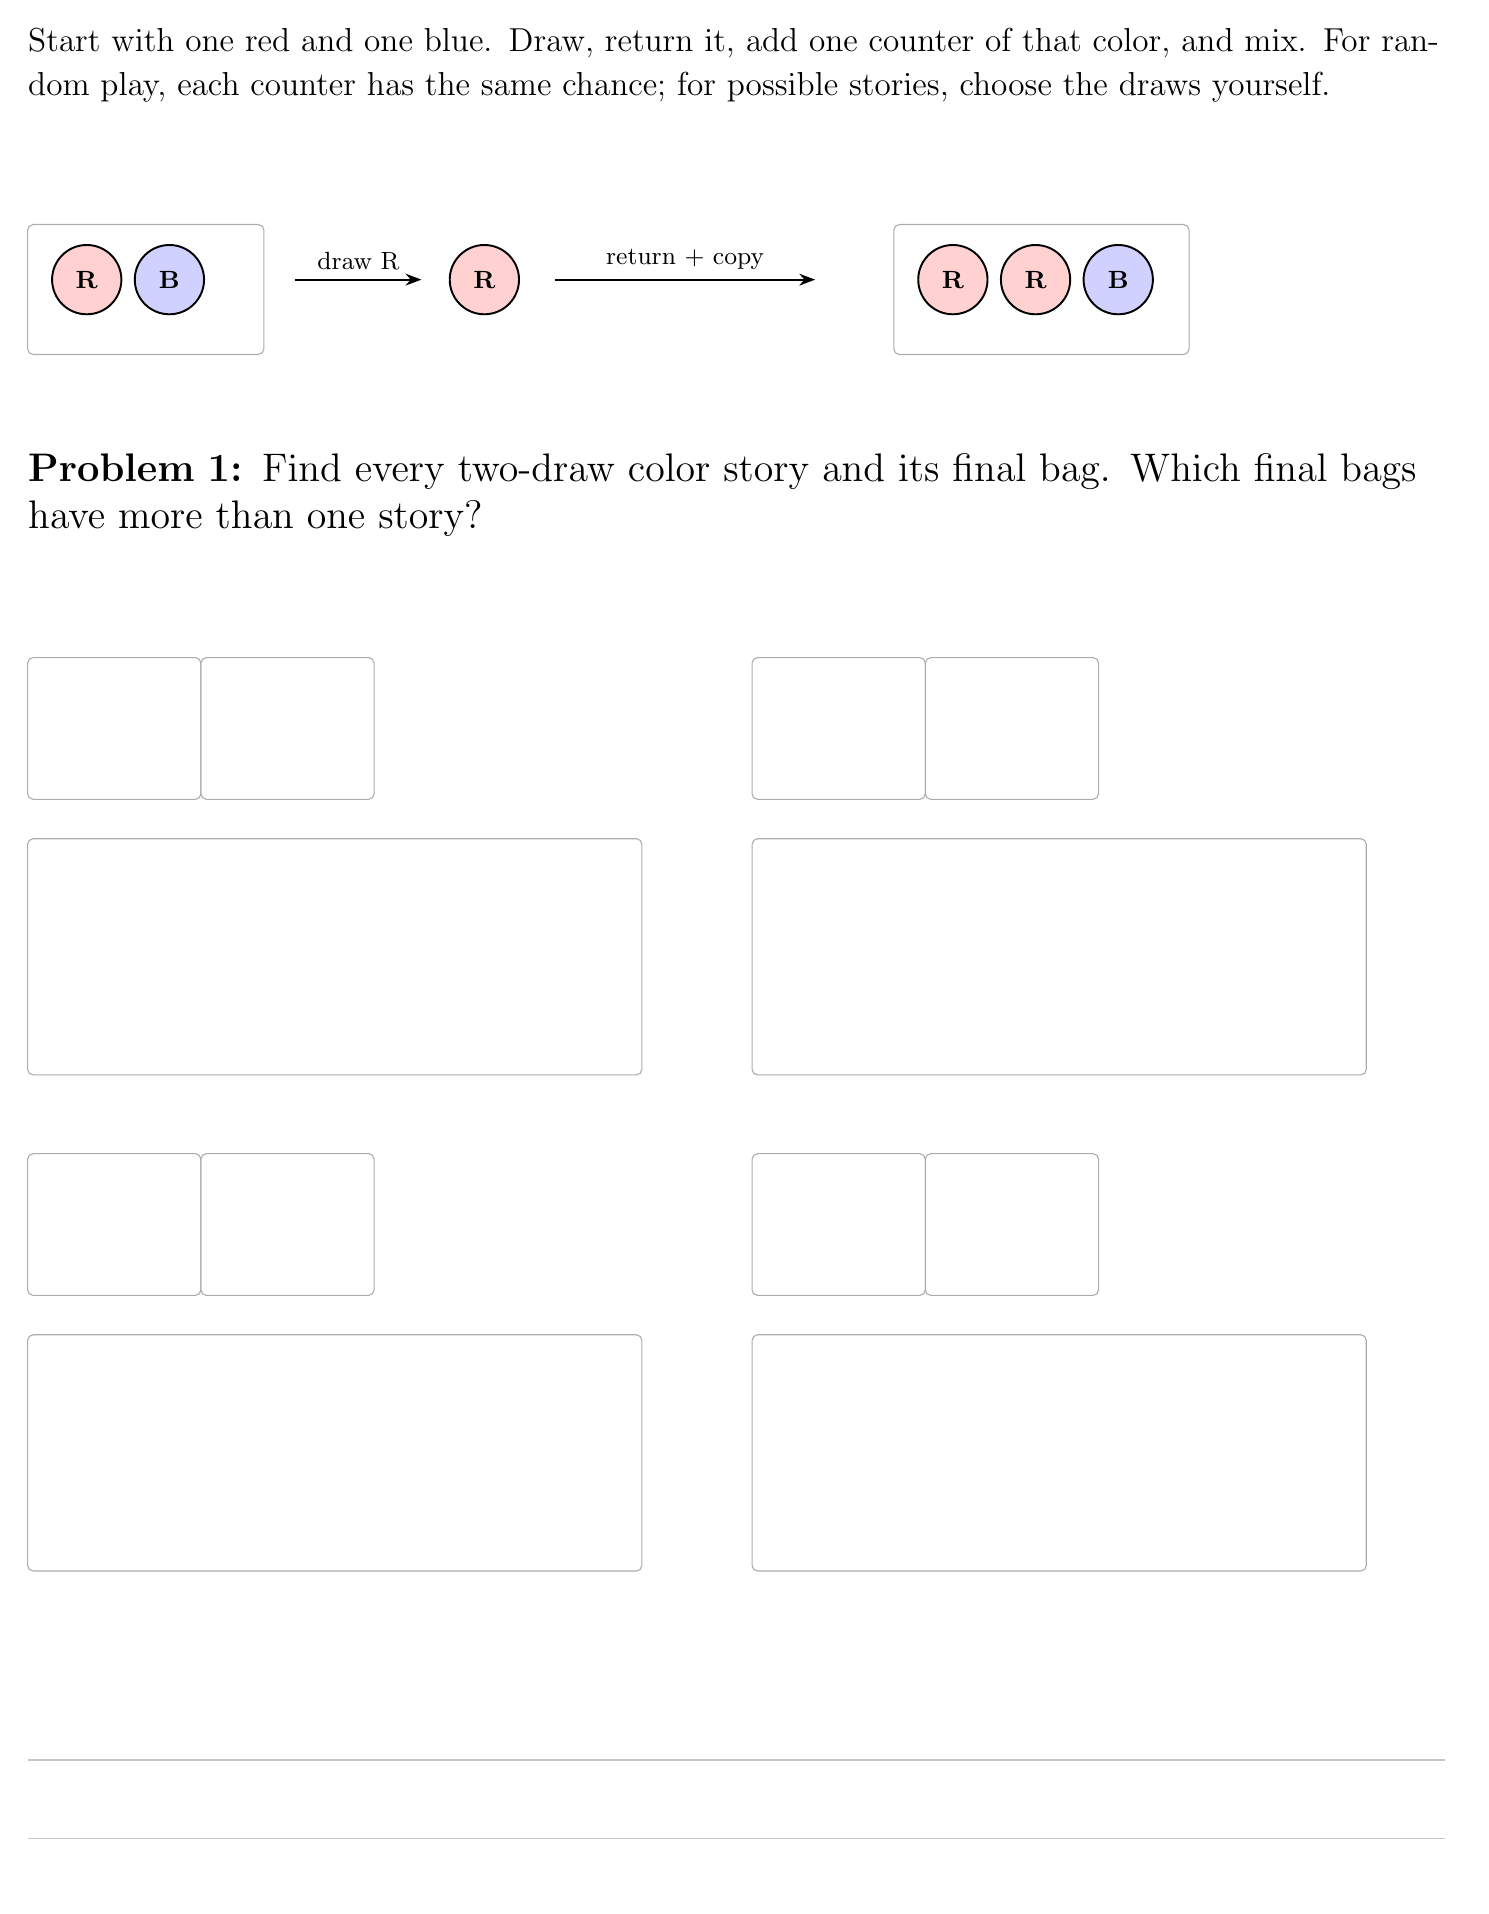
\begin{tikzpicture}[x=1cm,y=1cm]\path[use as bounding box] (0,0) rectangle (18.2,-23.6);
\node[anchor=north west,text width=18cm,inner sep=0pt,font=\fontsize{13}{16}\selectfont] at (0,0) {Start with one red and one blue. Draw, return it, add one counter of that color, and mix. For random play, each counter has the same chance; for possible stories, choose the draws yourself.};
\draw[gray!65,rounded corners=2pt] (0,-2.5) rectangle (3,-4.15);
\draw[fill=red!18,line width=.7pt] (0.75,-3.2) circle (0.44);
\node[font=\bfseries\small] at (0.75,-3.2) {R};
\draw[fill=blue!18,line width=.7pt] (1.8,-3.2) circle (0.44);
\node[font=\bfseries\small] at (1.8,-3.2) {B};
\draw[-{Stealth[length=2mm]},line width=.8pt] (3.4,-3.2) -- (5,-3.2) node[midway,above,font=\small] {draw R};
\draw[fill=red!18,line width=.7pt] (5.8,-3.2) circle (0.44);
\node[font=\bfseries\small] at (5.8,-3.2) {R};
\draw[-{Stealth[length=2mm]},line width=.8pt] (6.7,-3.2) -- (10,-3.2) node[midway,above,font=\small] {return + copy};
\draw[gray!65,rounded corners=2pt] (11,-2.5) rectangle (14.75,-4.15);
\draw[fill=red!18,line width=.7pt] (11.75,-3.2) circle (0.44);
\node[font=\bfseries\small] at (11.75,-3.2) {R};
\draw[fill=red!18,line width=.7pt] (12.8,-3.2) circle (0.44);
\node[font=\bfseries\small] at (12.8,-3.2) {R};
\draw[fill=blue!18,line width=.7pt] (13.85,-3.2) circle (0.44);
\node[font=\bfseries\small] at (13.85,-3.2) {B};
\node[anchor=north west,text width=18cm,inner sep=0pt,font=\fontsize{14}{17}\selectfont] at (0,-5.4) {\textbf{Problem 1:} Find every two-draw color story and its final bag. Which final bags have more than one story?};
\draw[gray!65,rounded corners=2pt] (0.0,-8.0) rectangle (2.2,-9.8);
\draw[gray!65,rounded corners=2pt] (2.2,-8.0) rectangle (4.4,-9.8);
\draw[gray!65,rounded corners=2pt] (0.0,-10.3) rectangle (7.8,-13.3);
\draw[gray!65,rounded corners=2pt] (9.2,-8.0) rectangle (11.399999999999999,-9.8);
\draw[gray!65,rounded corners=2pt] (11.399999999999999,-8.0) rectangle (13.599999999999998,-9.8);
\draw[gray!65,rounded corners=2pt] (9.2,-10.3) rectangle (17.0,-13.3);
\draw[gray!65,rounded corners=2pt] (0.0,-14.3) rectangle (2.2,-16.1);
\draw[gray!65,rounded corners=2pt] (2.2,-14.3) rectangle (4.4,-16.1);
\draw[gray!65,rounded corners=2pt] (0.0,-16.6) rectangle (7.8,-19.6);
\draw[gray!65,rounded corners=2pt] (9.2,-14.3) rectangle (11.399999999999999,-16.1);
\draw[gray!65,rounded corners=2pt] (11.399999999999999,-14.3) rectangle (13.599999999999998,-16.1);
\draw[gray!65,rounded corners=2pt] (9.2,-16.6) rectangle (17.0,-19.6);
\draw[gray!45] (0,-22) -- (18,-22);
\draw[gray!45] (0,-23) -- (18,-23);
\end{tikzpicture}
\newpage
\noindent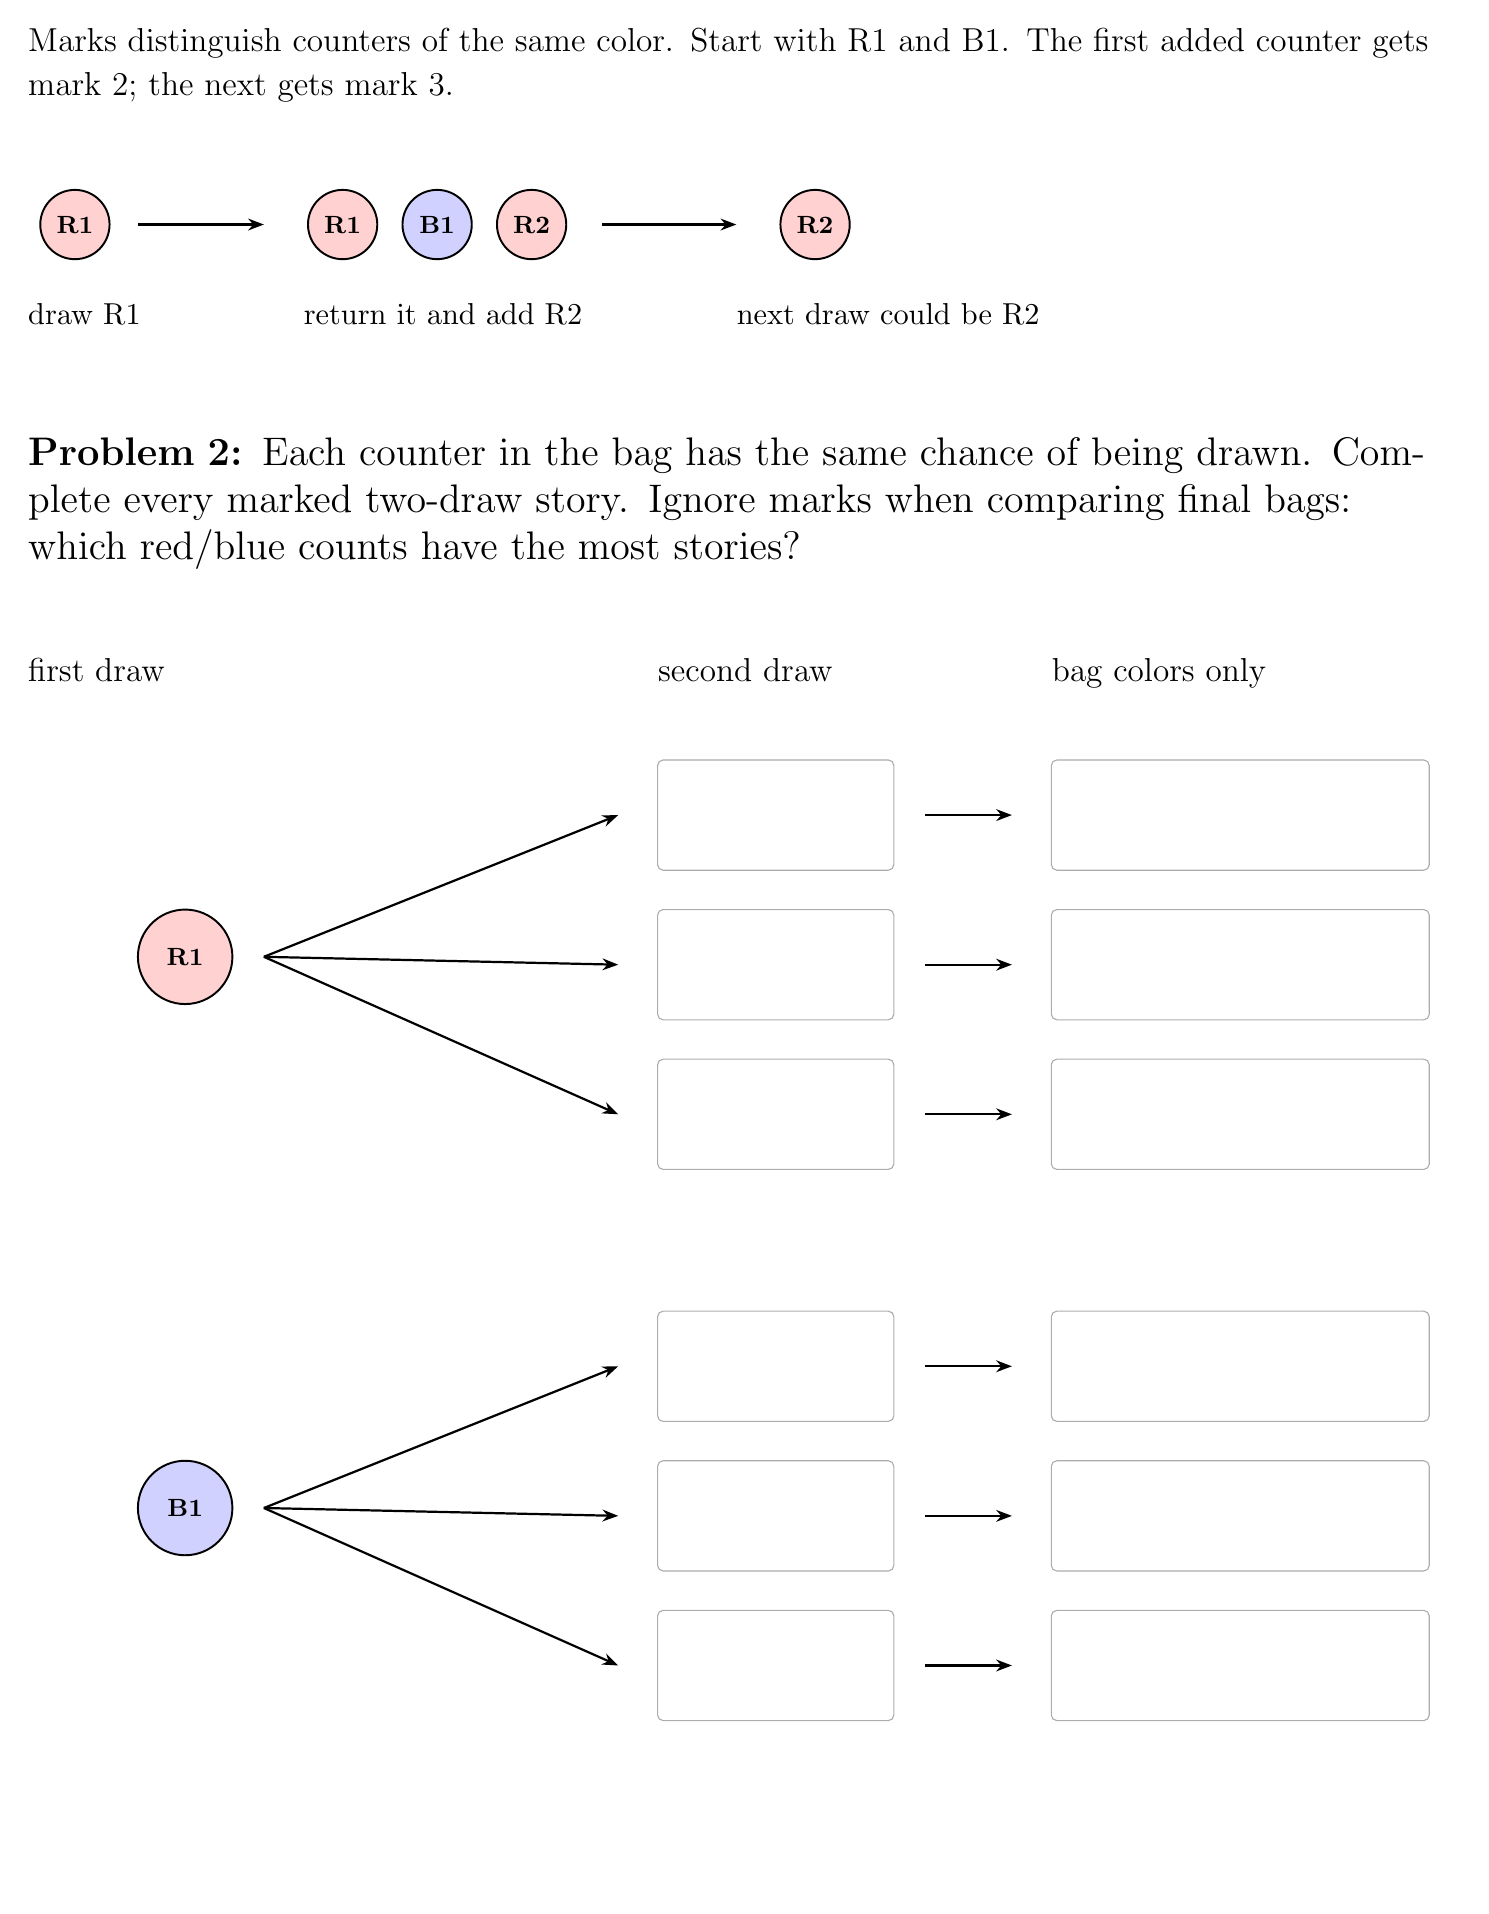
\begin{tikzpicture}[x=1cm,y=1cm]\path[use as bounding box] (0,0) rectangle (18.2,-23.6);
\node[anchor=north west,text width=18cm,inner sep=0pt,font=\fontsize{13}{16}\selectfont] at (0,0) {Marks distinguish counters of the same color. Start with R1 and B1. The first added counter gets mark 2; the next gets mark 3.};
\draw[fill=red!18,line width=.7pt] (0.6,-2.5) circle (0.44);
\node[font=\bfseries\small] at (0.6,-2.5) {R1};
\draw[-{Stealth[length=2mm]},line width=.8pt] (1.4,-2.5) -- (3,-2.5) node[midway,above,font=\small] {};
\draw[fill=red!18,line width=.7pt] (4,-2.5) circle (0.44);
\node[font=\bfseries\small] at (4,-2.5) {R1};
\draw[fill=blue!18,line width=.7pt] (5.2,-2.5) circle (0.44);
\node[font=\bfseries\small] at (5.2,-2.5) {B1};
\draw[fill=red!18,line width=.7pt] (6.4,-2.5) circle (0.44);
\node[font=\bfseries\small] at (6.4,-2.5) {R2};
\draw[-{Stealth[length=2mm]},line width=.8pt] (7.3,-2.5) -- (9,-2.5) node[midway,above,font=\small] {};
\draw[fill=red!18,line width=.7pt] (10,-2.5) circle (0.44);
\node[font=\bfseries\small] at (10,-2.5) {R2};
\node[anchor=north west,text width=3cm,inner sep=0pt,font=\fontsize{11}{14}\selectfont] at (0,-3.5) {draw R1};
\node[anchor=north west,text width=5cm,inner sep=0pt,font=\fontsize{11}{14}\selectfont] at (3.5,-3.5) {return it and add R2};
\node[anchor=north west,text width=8cm,inner sep=0pt,font=\fontsize{11}{14}\selectfont] at (9,-3.5) {next draw could be R2};
\node[anchor=north west,text width=18cm,inner sep=0pt,font=\fontsize{14}{17}\selectfont] at (0,-5.2) {\textbf{Problem 2:} Each counter in the bag has the same chance of being drawn. Complete every marked two-draw story. Ignore marks when comparing final bags: which red/blue counts have the most stories?};
\node[anchor=north west,text width=3cm,inner sep=0pt,font=\fontsize{12}{15}\selectfont] at (0,-8) {first draw};
\node[anchor=north west,text width=5cm,inner sep=0pt,font=\fontsize{12}{15}\selectfont] at (8,-8) {second draw};
\node[anchor=north west,text width=4.8cm,inner sep=0pt,font=\fontsize{12}{15}\selectfont] at (13,-8) {bag colors only};
\draw[fill=red!18,line width=.7pt] (2,-11.8) circle (0.6);
\node[font=\bfseries\small] at (2,-11.8) {R1};
\draw[-{Stealth[length=2mm]},line width=.8pt] (3,-11.8) -- (7.5,-10.0) node[midway,above,font=\small] {};
\draw[gray!65,rounded corners=2pt] (8,-9.3) rectangle (11,-10.700000000000001);
\draw[-{Stealth[length=2mm]},line width=.8pt] (11.4,-10.0) -- (12.5,-10.0) node[midway,above,font=\small] {};
\draw[gray!65,rounded corners=2pt] (13,-9.3) rectangle (17.8,-10.700000000000001);
\draw[-{Stealth[length=2mm]},line width=.8pt] (3,-11.8) -- (7.5,-11.9) node[midway,above,font=\small] {};
\draw[gray!65,rounded corners=2pt] (8,-11.200000000000001) rectangle (11,-12.600000000000001);
\draw[-{Stealth[length=2mm]},line width=.8pt] (11.4,-11.9) -- (12.5,-11.9) node[midway,above,font=\small] {};
\draw[gray!65,rounded corners=2pt] (13,-11.200000000000001) rectangle (17.8,-12.600000000000001);
\draw[-{Stealth[length=2mm]},line width=.8pt] (3,-11.8) -- (7.5,-13.8) node[midway,above,font=\small] {};
\draw[gray!65,rounded corners=2pt] (8,-13.100000000000001) rectangle (11,-14.500000000000002);
\draw[-{Stealth[length=2mm]},line width=.8pt] (11.4,-13.8) -- (12.5,-13.8) node[midway,above,font=\small] {};
\draw[gray!65,rounded corners=2pt] (13,-13.100000000000001) rectangle (17.8,-14.500000000000002);
\draw[fill=blue!18,line width=.7pt] (2,-18.8) circle (0.6);
\node[font=\bfseries\small] at (2,-18.8) {B1};
\draw[-{Stealth[length=2mm]},line width=.8pt] (3,-18.8) -- (7.5,-17.0) node[midway,above,font=\small] {};
\draw[gray!65,rounded corners=2pt] (8,-16.3) rectangle (11,-17.7);
\draw[-{Stealth[length=2mm]},line width=.8pt] (11.4,-17.0) -- (12.5,-17.0) node[midway,above,font=\small] {};
\draw[gray!65,rounded corners=2pt] (13,-16.3) rectangle (17.8,-17.7);
\draw[-{Stealth[length=2mm]},line width=.8pt] (3,-18.8) -- (7.5,-18.9) node[midway,above,font=\small] {};
\draw[gray!65,rounded corners=2pt] (8,-18.2) rectangle (11,-19.599999999999998);
\draw[-{Stealth[length=2mm]},line width=.8pt] (11.4,-18.9) -- (12.5,-18.9) node[midway,above,font=\small] {};
\draw[gray!65,rounded corners=2pt] (13,-18.2) rectangle (17.8,-19.599999999999998);
\draw[-{Stealth[length=2mm]},line width=.8pt] (3,-18.8) -- (7.5,-20.8) node[midway,above,font=\small] {};
\draw[gray!65,rounded corners=2pt] (8,-20.1) rectangle (11,-21.5);
\draw[-{Stealth[length=2mm]},line width=.8pt] (11.4,-20.8) -- (12.5,-20.8) node[midway,above,font=\small] {};
\draw[gray!65,rounded corners=2pt] (13,-20.1) rectangle (17.8,-21.5);
\end{tikzpicture}
\newpage
\noindent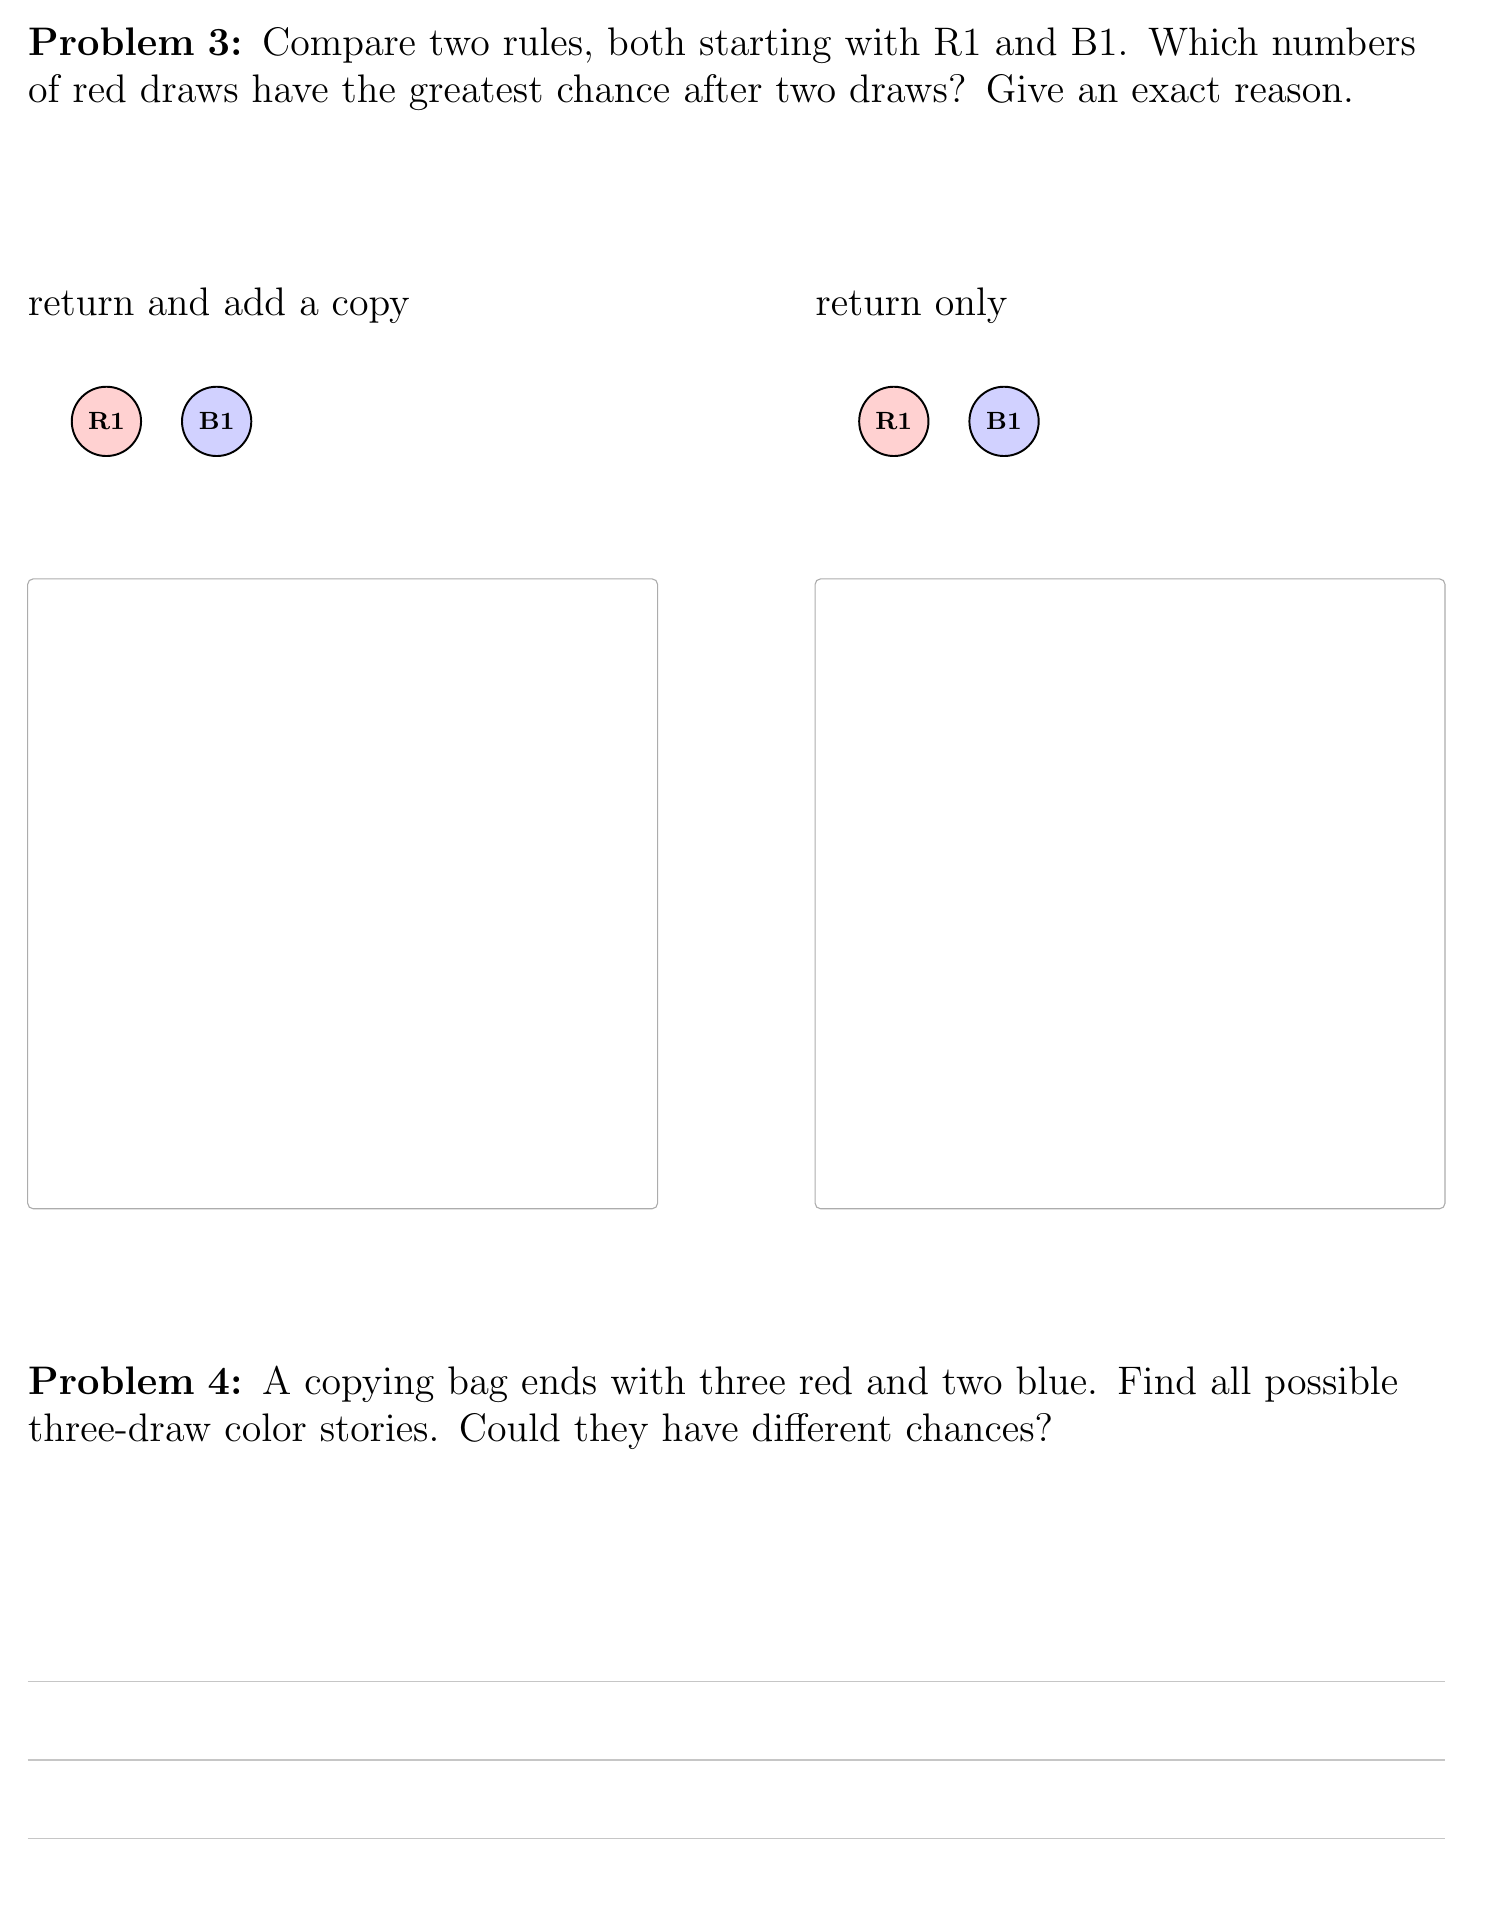
\begin{tikzpicture}[x=1cm,y=1cm]\path[use as bounding box] (0,0) rectangle (18.2,-23.6);
\node[anchor=north west,text width=18cm,inner sep=0pt,font=\fontsize{14}{17}\selectfont] at (0,0) {\textbf{Problem 3:} Compare two rules, both starting with R1 and B1. Which numbers of red draws have the greatest chance after two draws? Give an exact reason.};
\node[anchor=north west,text width=8cm,inner sep=0pt,font=\fontsize{14}{17}\selectfont] at (0,-3.3) {return and add a copy};
\node[anchor=north west,text width=8cm,inner sep=0pt,font=\fontsize{14}{17}\selectfont] at (10,-3.3) {return only};
\draw[fill=red!18,line width=.7pt] (1,-5) circle (0.44);
\node[font=\bfseries\small] at (1,-5) {R1};
\draw[fill=blue!18,line width=.7pt] (2.4,-5) circle (0.44);
\node[font=\bfseries\small] at (2.4,-5) {B1};
\draw[gray!65,rounded corners=2pt] (0,-7) rectangle (8,-15);
\draw[fill=red!18,line width=.7pt] (11,-5) circle (0.44);
\node[font=\bfseries\small] at (11,-5) {R1};
\draw[fill=blue!18,line width=.7pt] (12.4,-5) circle (0.44);
\node[font=\bfseries\small] at (12.4,-5) {B1};
\draw[gray!65,rounded corners=2pt] (10,-7) rectangle (18,-15);
\node[anchor=north west,text width=18cm,inner sep=0pt,font=\fontsize{14}{17}\selectfont] at (0,-17) {\textbf{Problem 4:} A copying bag ends with three red and two blue. Find all possible three-draw color stories. Could they have different chances?};
\draw[gray!45] (0,-21) -- (18,-21);
\draw[gray!45] (0,-22) -- (18,-22);
\draw[gray!45] (0,-23) -- (18,-23);
\end{tikzpicture}
\newpage
\noindent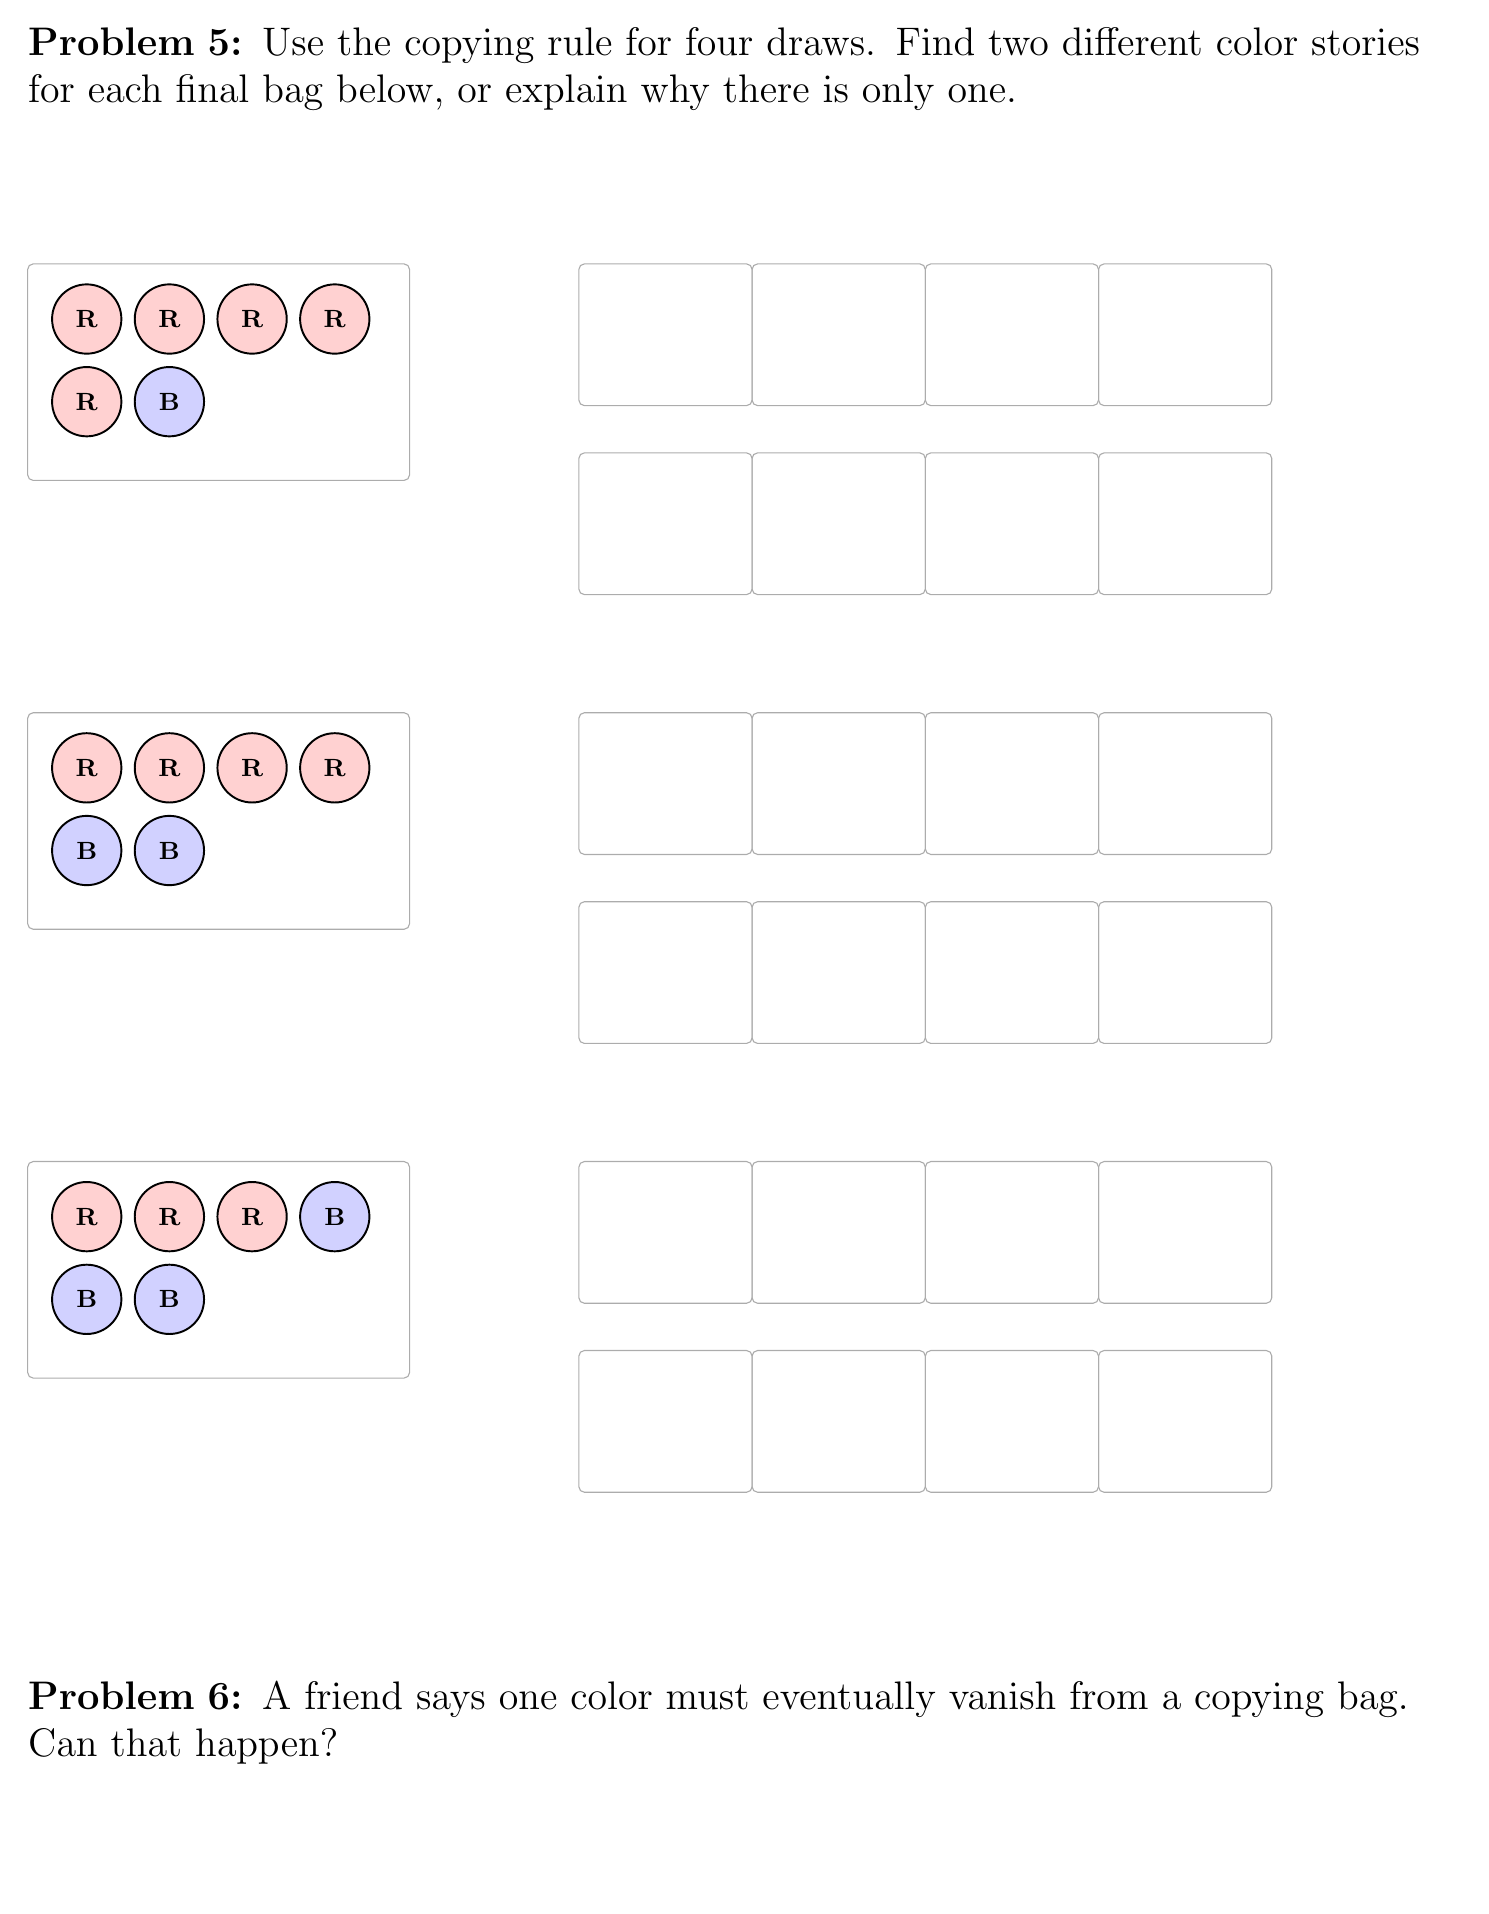
\begin{tikzpicture}[x=1cm,y=1cm]\path[use as bounding box] (0,0) rectangle (18.2,-23.6);
\node[anchor=north west,text width=18cm,inner sep=0pt,font=\fontsize{14}{17}\selectfont] at (0,0) {\textbf{Problem 5:} Use the copying rule for four draws. Find two different color stories for each final bag below, or explain why there is only one.};
\draw[gray!65,rounded corners=2pt] (0,-3.0) rectangle (4.8500000000000005,-5.75);
\draw[fill=red!18,line width=.7pt] (0.75,-3.7) circle (0.44);
\node[font=\bfseries\small] at (0.75,-3.7) {R};
\draw[fill=red!18,line width=.7pt] (1.8,-3.7) circle (0.44);
\node[font=\bfseries\small] at (1.8,-3.7) {R};
\draw[fill=red!18,line width=.7pt] (2.85,-3.7) circle (0.44);
\node[font=\bfseries\small] at (2.85,-3.7) {R};
\draw[fill=red!18,line width=.7pt] (3.9000000000000004,-3.7) circle (0.44);
\node[font=\bfseries\small] at (3.9000000000000004,-3.7) {R};
\draw[fill=red!18,line width=.7pt] (0.75,-4.75) circle (0.44);
\node[font=\bfseries\small] at (0.75,-4.75) {R};
\draw[fill=blue!18,line width=.7pt] (1.8,-4.75) circle (0.44);
\node[font=\bfseries\small] at (1.8,-4.75) {B};
\draw[gray!65,rounded corners=2pt] (7.0,-3.0) rectangle (9.2,-4.8);
\draw[gray!65,rounded corners=2pt] (9.2,-3.0) rectangle (11.399999999999999,-4.8);
\draw[gray!65,rounded corners=2pt] (11.4,-3.0) rectangle (13.600000000000001,-4.8);
\draw[gray!65,rounded corners=2pt] (13.600000000000001,-3.0) rectangle (15.8,-4.8);
\draw[gray!65,rounded corners=2pt] (7.0,-5.4) rectangle (9.2,-7.2);
\draw[gray!65,rounded corners=2pt] (9.2,-5.4) rectangle (11.399999999999999,-7.2);
\draw[gray!65,rounded corners=2pt] (11.4,-5.4) rectangle (13.600000000000001,-7.2);
\draw[gray!65,rounded corners=2pt] (13.600000000000001,-5.4) rectangle (15.8,-7.2);
\draw[gray!65,rounded corners=2pt] (0,-8.7) rectangle (4.8500000000000005,-11.45);
\draw[fill=red!18,line width=.7pt] (0.75,-9.399999999999999) circle (0.44);
\node[font=\bfseries\small] at (0.75,-9.399999999999999) {R};
\draw[fill=red!18,line width=.7pt] (1.8,-9.399999999999999) circle (0.44);
\node[font=\bfseries\small] at (1.8,-9.399999999999999) {R};
\draw[fill=red!18,line width=.7pt] (2.85,-9.399999999999999) circle (0.44);
\node[font=\bfseries\small] at (2.85,-9.399999999999999) {R};
\draw[fill=red!18,line width=.7pt] (3.9000000000000004,-9.399999999999999) circle (0.44);
\node[font=\bfseries\small] at (3.9000000000000004,-9.399999999999999) {R};
\draw[fill=blue!18,line width=.7pt] (0.75,-10.45) circle (0.44);
\node[font=\bfseries\small] at (0.75,-10.45) {B};
\draw[fill=blue!18,line width=.7pt] (1.8,-10.45) circle (0.44);
\node[font=\bfseries\small] at (1.8,-10.45) {B};
\draw[gray!65,rounded corners=2pt] (7.0,-8.7) rectangle (9.2,-10.5);
\draw[gray!65,rounded corners=2pt] (9.2,-8.7) rectangle (11.399999999999999,-10.5);
\draw[gray!65,rounded corners=2pt] (11.4,-8.7) rectangle (13.600000000000001,-10.5);
\draw[gray!65,rounded corners=2pt] (13.600000000000001,-8.7) rectangle (15.8,-10.5);
\draw[gray!65,rounded corners=2pt] (7.0,-11.1) rectangle (9.2,-12.9);
\draw[gray!65,rounded corners=2pt] (9.2,-11.1) rectangle (11.399999999999999,-12.9);
\draw[gray!65,rounded corners=2pt] (11.4,-11.1) rectangle (13.600000000000001,-12.9);
\draw[gray!65,rounded corners=2pt] (13.600000000000001,-11.1) rectangle (15.8,-12.9);
\draw[gray!65,rounded corners=2pt] (0,-14.4) rectangle (4.8500000000000005,-17.15);
\draw[fill=red!18,line width=.7pt] (0.75,-15.1) circle (0.44);
\node[font=\bfseries\small] at (0.75,-15.1) {R};
\draw[fill=red!18,line width=.7pt] (1.8,-15.1) circle (0.44);
\node[font=\bfseries\small] at (1.8,-15.1) {R};
\draw[fill=red!18,line width=.7pt] (2.85,-15.1) circle (0.44);
\node[font=\bfseries\small] at (2.85,-15.1) {R};
\draw[fill=blue!18,line width=.7pt] (3.9000000000000004,-15.1) circle (0.44);
\node[font=\bfseries\small] at (3.9000000000000004,-15.1) {B};
\draw[fill=blue!18,line width=.7pt] (0.75,-16.15) circle (0.44);
\node[font=\bfseries\small] at (0.75,-16.15) {B};
\draw[fill=blue!18,line width=.7pt] (1.8,-16.15) circle (0.44);
\node[font=\bfseries\small] at (1.8,-16.15) {B};
\draw[gray!65,rounded corners=2pt] (7.0,-14.4) rectangle (9.2,-16.2);
\draw[gray!65,rounded corners=2pt] (9.2,-14.4) rectangle (11.399999999999999,-16.2);
\draw[gray!65,rounded corners=2pt] (11.4,-14.4) rectangle (13.600000000000001,-16.2);
\draw[gray!65,rounded corners=2pt] (13.600000000000001,-14.4) rectangle (15.8,-16.2);
\draw[gray!65,rounded corners=2pt] (7.0,-16.8) rectangle (9.2,-18.6);
\draw[gray!65,rounded corners=2pt] (9.2,-16.8) rectangle (11.399999999999999,-18.6);
\draw[gray!65,rounded corners=2pt] (11.4,-16.8) rectangle (13.600000000000001,-18.6);
\draw[gray!65,rounded corners=2pt] (13.600000000000001,-16.8) rectangle (15.8,-18.6);
\node[anchor=north west,text width=18cm,inner sep=0pt,font=\fontsize{14}{17}\selectfont] at (0,-21) {\textbf{Problem 6:} A friend says one color must eventually vanish from a copying bag. Can that happen?};
\end{tikzpicture}
\end{document}
